\part{无穷级数}
\section{数项级数}
一个给定的数列$a_1,a_2,\cdots,a_n,\cdots$的求和
\[ \sum_{n=1}^\infty a_n = a_1 + a_2 + \cdots + a_n + \cdots \]
称为\textcolor{red}{\textbf{\textsf{数项级数}}},其前$n$项和
\[ S_n = a_1 + a_2 + \cdots a_n \]
称为$\displaystyle \sum_{n=1}^\infty a_n$的\textcolor{red}{\textbf{\textsf{部分和}}}。

\subsection{级数的敛散性}
若部分和$S_n$的极限为$S$,则称级数$\displaystyle\sum_{n=1}^\infty a_n$收敛于$S$,
由此可得数项级数的基本性质
\begin{enumerate}[itemindent=1em,label=\textbf{\textsf{性质}}\arabic*]
    \item 若$k\neq 0$,则级数$\displaystyle\sum_{n=1}^\infty ka_n$与$\displaystyle\sum_{n=1}^\infty a_n$
          的敛散性相同且
          \[ \sum_{n=1}^\infty ka_n = k\sum_{n=1}^\infty a_n \]
    \item 改变级数的有限项不改变级数的敛散性
    \item 收敛级数的和差级数为收敛级数,即
          \[ \sum_{n=1}^\infty a_n \pm \sum_{n=1}^\infty b_n = \sum_{n=1}^\infty (a_n\pm b_n) \]
    \item 收敛级数的加括号级数为收敛级数
    \item 收敛级数的通项极限必为零,即$\displaystyle\sum_{n=1}^\infty a_n$收敛时,必有
          \[ \lim_{n\to\infty} a_n = 0 \]
\end{enumerate}

\subsection{正项级数}
若级数的每一项都非负,则称级数为\textcolor{red}{\textbf{\textsf{正项级数}}},根据数列极限的单调有界法则\ref{th:单调有界法则}可知,
正项级数收敛当且仅当它的部分和数列有界(正项级数部分和是递增的)。

\begin{theorem}
    (积分判别法)
    \label{th:积分判别法}
    若函数$f(x)$是区间$[1,+\infty)$上的非负递减函数,则
    \[ \sum_{n=1}^\infty f(n)\text{ 收敛} \iff \int_1^{+\infty}f(x)\,\diff x\text{ 收敛}\]
\end{theorem}

\begin{theorem}
    (比较判别法)
    \label{th:级数比较判别法}
    设$\displaystyle\sum_{n=1}^\infty u_n,\sum_{n=1}^\infty v_n$为正项级数且恒有$u_n\leq v_n$,则
    \begin{enumerate}[(1)]
        \item $\displaystyle \sum_{n=1}^\infty v_n\text{ 收敛}\implies\sum_{n=1}^\infty u_n\text{ 收敛}$;(大级数收敛小收敛)
        \item $\displaystyle \sum_{n=1}^\infty u_n\text{ 发散}\implies\sum_{n=1}^\infty v_n\text{ 发散}$。(小级数发散大发散)
    \end{enumerate}
    推论:
    若$n\to\infty$时,恒有$u_n\leq kv_n$,若$k\neq 0$,则有
    \begin{enumerate}[(1)]
        \item $\displaystyle \sum_{n=1}^\infty v_n\text{ 收敛}\implies\sum_{n=1}^\infty u_n\text{ 收敛}$;
        \item $\displaystyle \sum_{n=1}^\infty u_n\text{ 发散}\implies\sum_{n=1}^\infty v_n\text{ 发散}$。
    \end{enumerate}
\end{theorem}

\begin{theorem}
    (极限判别法)
    \label{th:级数极限判别法}
    设$\displaystyle\sum_{n=1}^\infty u_n,\sum_{n=1}^\infty v_n$为正项级数,若$\displaystyle\lim_{n\to\infty}\frac{u_n}{v_n}=A$,则
    \begin{enumerate}[(1)]
        \item 当$0<A<+\infty$时,即$u_n\sim Av_n$,$\displaystyle\sum_{n=1}^\infty u_n$与$\displaystyle\sum_{n=1}^\infty v_n$同时收敛同时发散;
        \item 当$A=0$时,$\displaystyle\sum_{n=1}^\infty u_n\text{ 发散}\implies\sum_{n=1}^\infty v_n\text{ 发散}$。
        \item 当$A=+\infty$时,$\displaystyle\sum_{n=1}^\infty v_n\text{ 收敛}\implies\sum_{n=1}^\infty u_n\text{ 收敛}$。
    \end{enumerate}
\end{theorem}

\begin{example}
    判断下列级数的敛散性
    \begin{tasks}[label=(\arabic*),label-width = 2em](3)
        \task $\displaystyle \sum_{n=1}^\infty \sin\frac{1}{n}$
        \task $\displaystyle \sum_{n=1}^\infty \ln\left(1+\frac{1}{n^2}\right)$
        \task $\displaystyle \sum_{n=1}^\infty \frac{1}{\sqrt{n(n+1)}}$
    \end{tasks}
\end{example}
\begin{solution}
    由于$n\to\infty$时,
    \[
        \sin\frac{1}{n} \sim \frac{1}{n}, \qquad
        \ln\left(1+\frac{1}{n^2}\right) \sim \frac{1}{n^2}, \qquad
        \frac{1}{\sqrt{n(n+1)}} \sim \frac{1}{n}
    \]
    所以
    $\displaystyle \sum_{n=1}^\infty \sin\frac{1}{n}$发散,
    $\displaystyle \sum_{n=1}^\infty \ln\left(1+\frac{1}{n^2}\right)$收敛,
    $\displaystyle \sum_{n=1}^\infty \frac{1}{\sqrt{n(n+1)}}$发散。
\end{solution}

\marginnote{
    比值判别法、根值判别法中无法通过$l=1$来判别级数的敛散性,例如下面两个级数
    \[ \sum_{n=1}^\infty \frac{1}{n^2} \qquad \sum_{n=1}^\infty 1 \]
    $l$均为$1$,但是前者收敛,后者发散。
}
\begin{theorem}
    (比值判别法)
    \label{th:比值判别法}
    设$\displaystyle\sum_{n=1}^\infty u_n$为正项级数,若$\displaystyle\lim_{n\to\infty}\frac{u_{n+1}}{u_n}=l$,则
    \begin{enumerate}[(1)]
        \item 当$l<1$时,$\displaystyle\sum_{n=1}^\infty u_n$收敛。
        \item 当$l>1$时,$\displaystyle\sum_{n=1}^\infty u_n$发散。
    \end{enumerate}
\end{theorem}
\begin{theorem}
    (根值判别法)
    \label{th:根值判别法}
    设$\displaystyle\sum_{n=1}^\infty u_n$为正项级数,若$\displaystyle\lim_{n\to\infty}\sqrt[n]{u_n}=l$,则
    \begin{enumerate}[(1)]
        \item 当$l<1$时,$\displaystyle\sum_{n=1}^\infty u_n$收敛。
        \item 当$l>1$时,$\displaystyle\sum_{n=1}^\infty u_n$发散。
    \end{enumerate}
\end{theorem}

\begin{example}
    判断下列级数的敛散性
    \begin{tasks}[label=(\arabic*),label-width = 2em](2)
        \task $\displaystyle \sum_{n=1}^\infty \frac{n!x^n}{n^n}\,(x>0)$
        \task $\displaystyle \sum_{n=1}^\infty \frac{n^k}{2^n}\,(k>0)$
        \task $\displaystyle \sum_{n=1}^\infty \left(\frac{n}{2n+1}\right)^n$
        \task $\displaystyle \sum_{n=1}^\infty nx^n\,(x>0)$
    \end{tasks}
\end{example}
\begin{solution}
    \begin{enumerate}[(1)]
        \item 根据比值判别法
              \[ \lim_{n\to\infty} \frac{u_{n+1}}{u_n} = \lim_{n\to\infty} \left(\frac{n}{n+1}\right)^{n}x = \frac{x}{e}\]
              所以当$x<e$时,原级数收敛,$x>e$时原级数发散。
        \item 根据比值判别法
              \[
                  \lim_{n\to\infty} \frac{\left.(n+1)^k\middle/2^{n+1}\right.}{\left.n^k\middle/2^{n}\right.}
                  =
                  \frac{1}{2}\lim_{n\to\infty} \left(1+\frac{1}{n}\right)^k
                  =
                  \frac{1}{2}
              \]
              所以原级数收敛。
        \item 根据根值判别法
              \[
                  \lim_{n\to\infty} \sqrt[n]{\left(\frac{n}{2n+1}\right)^n}
                  =
                  \lim_{n\to\infty} \frac{n}{2n+1}
                  =
                  \frac{1}{2}
              \]
              所以原级数收敛。
        \item 根据根值判别法
              \[ \lim_{n\to\infty} \sqrt[n]{nx^n} = x \]
              当$x<1$时,原级数收;当$x>1$时,原级数发散;当$x=1$时,级数为$\displaystyle\sum_{n=1}^\infty n$,发散。
    \end{enumerate}
\end{solution}

\subsection{任意项级数}
一般项级数的敛散性常用有限片段的方法研究,即数列极限的柯西准则\ref{th:柯西准则}。
级数的部分和$S_n$,根据柯西准则,当$\forall \varepsilon > 0,\exists N$,使得当$m>n>N$时,恒有
$|S_m-S_n|<\varepsilon$,即
\[ \left|\sum_{k\geq n}^m u_k \right|<\varepsilon \]


形如$u_1 - u_2 + \cdots + (-1)^{n+1}u_n + \cdots$或$-u_1 + u_2 - \cdots + (-1)^n u_n + \cdots$
的级数称为\textcolor{red}{\textbf{\textsf{交错级数}}}。其中$u_1,u_2,\cdots,u_n\cdots$均为正数。
对于交错级数,通常使用Leibniz判别法确定收敛性。
\begin{theorem}
    (Leibniz判别法)
    \label{th:Leibniz判别法}
    如果教材级数$\displaystyle\sum_{n=1}^\infty(-1)^n u_n$的绝对通项$u_n$单调趋于$0$,
    即$u_n>u_{n_1}\to 0(n\to\infty)$,则该级数收敛。
\end{theorem}

一个级数$\displaystyle\sum_{n=1}^\infty u_n$的\textcolor{red}{\textbf{\textsf{绝对化级数}}}
$\displaystyle\sum_{n=1}^\infty |u_n|$收敛,则称该级数\textcolor{red}{\textbf{\textsf{绝对收敛}}};
一个收敛的级数的绝对化级数发散,则称该级数\textcolor{red}{\textbf{\textsf{条件收敛}}}。
\sidenote{
    绝对化级数收敛$\implies$绝对收敛\\
    \textcolor{red}{收敛}的级数,若它的绝对化级数发散$\implies$条件收敛
}

\begin{theorem}
    (绝对收敛法)
    \label{th:绝对收敛法}
    绝对收敛级数一定收敛。
    \[ \sum_{n=1}^\infty |u_n|\text{ 收敛}\implies \sum_{n=1}^\infty u_n \text{ 收敛} \]
\end{theorem}

\begin{example}
    设$u_n=\dfrac{(-x)^n}{n^p},(x>0,p>0)$,讨论级数$\displaystyle\sum_{n=1}^\infty u_n$的敛散性。
\end{example}
\begin{solution}
    根据比值判别法,
    \[
        \lim_{n\to\infty} \frac{|u_{n+1}|}{|u_n|}
        =
        \lim_{n\to\infty} x\left(\frac{n}{n+1}\right)^p
        =
        x
    \]
    当$x<1$时,原级数绝对收敛;

    当$x>1$时,$\displaystyle\lim_{n\to\infty}|u_n|=\lim_{n\to\infty}\frac{x^n}{n^p}=+\infty$,
    所以原级数发散;

    当$x=1$时,若$p>1$,则$\displaystyle\sum_{n=0}^\infty u_n$绝对收敛,若$p\leq 1$,根据Leibniz判别法,$\displaystyle\sum_{n=0}^\infty u_n$条件收敛。
\end{solution}

\begin{example}
    若函数$f(x)$在$x=0$的某领域内具有连续的二阶导数,且$\displaystyle\lim_{x\to 0}\frac{f(x)}{x} = 0$,
    试证$\displaystyle\sum_{n=1}^\infty f\left(\frac{1}{n}\right)$绝对收敛。
\end{example}
\begin{proof}
    根据泰勒公式和二阶导数的有界性,以及比较判别法,易证命题。下面使用极限判别法来证明。
    由于$f(x)$存在连续二阶导数,且$\displaystyle\lim_{x\to 0}\frac{f(x)}{x} = 0$,所以$f(0)=f'(0)=0$
    那么有
    \[
        \lim_{n\to\infty} \frac{\left|f\left(\frac{1}{n}\right)\right|}{\frac{1}{n^2}}
        =
        \lim_{x\to 0^+}\left|\frac{f(x)}{x^2}\right|
        =
        \lim_{x\to0^+} \left|\frac{f'(x)}{2x}\right|
        =
        \frac{1}{2}|f''(0)|
    \]
    因为$\displaystyle\sum_{n=1}^\infty\frac{1}{n^2}$收敛,
    所以$\displaystyle\sum_{n=1}^\infty f\left(\frac{1}{n}\right)$绝对收敛。
\end{proof}

\begin{example}
    判别级数$\displaystyle\sum_{n=1}^\infty \sin(\pi\sqrt{n^2+a^2})$的敛散性。
\end{example}
\begin{solution}
    \[
        \sin(\pi\sqrt{n^2+a^2})
        = \sin\left[n\pi + \pi\left(\sqrt{n^2+a^2} - n\right)\right]
        = (-1)^n\sin\frac{a^2\pi}{\sqrt{n^2+a^2}+n}
    \]
    当$n$充分大时$\left\{\sin\dfrac{a^2\pi}{\sqrt{n^2+a^2}+n}\right\}$,单调减且趋于$0$,
    根据Leibniz判别法可知原级数收敛。
\end{solution}

\begin{example}
    判断级数$\displaystyle\sum_{n=1}^\infty \ln \left[1+\frac{(-1)^n}{\sqrt{n}}\right]$的敛散性。
\end{example}
\begin{solution}
    根据泰勒公式,
    \[ \ln \left[1+\frac{(-1)^n}{\sqrt{n}}\right] = \frac{(-1)^n}{\sqrt{n}} - \frac{1}{2n} + o\left(\frac{1}{n}\right) \]
    根据Leibniz判别法,级数$\displaystyle\sum_{n=1}^\infty \frac{(-1)^n}{\sqrt{n}}$收敛。

    而根据极限判别法
    \[ \lim_{n\to\infty} \frac{\frac{1}{2n}-o\left(\frac{1}{n}\right)}{\frac{1}{n}} = \frac{1}{2} \]
    故级数$\displaystyle\sum_{n=1}^\infty \frac{1}{2n}-o\left(\frac{1}{n}\right)$发散。

    所以原级数发散。
\end{solution}

\begin{example}
    判断级数级数$\displaystyle\sum_{n=2}^\infty \frac{(-1)^n}{\sqrt{n}+(-1)^n}$的敛散性。
\end{example}
\begin{solution}
    \[
        \frac{(-1)^n}{\sqrt{n}+(-1)^n}
        =
        \frac{(-1)^n\left(\sqrt{n}-(-1)^n\right)}{n-1}
        =
        \frac{(-1)^n\sqrt{n}-1}{n-1}
        =
        (-1)^n\frac{\sqrt{n}}{n-1} - \frac{1}{n-1}
    \]
    设$f(x)=\dfrac{\sqrt{x}}{x-1}, (x\geq 2)$,显然$f(x)>0$,且
    \[
        f'(x)
        = \frac{\frac{1}{2\sqrt{x}}(x-1) - \sqrt{x}}{(x-1)^2}
        = -\frac{x+1}{2\sqrt{x}(x-1)^2}<0
    \]
    则函数$f(x)$单调递减,根据Leibniz判别法级数$\displaystyle\sum_{n=2}^\infty (-1)^n\frac{\sqrt{n}}{n-1}$收敛,
    而$\displaystyle\sum_{n=2}^\infty \frac{1}{n-1}$发散,所以原级数发散。
\end{solution}

\begin{example}
    证明:级数$\displaystyle\sum_{n=2}^\infty \frac{(-1)^n}{\sqrt{n + (-1)^n}}$条件收敛。
\end{example}
\begin{proof}
    \[
        S_{2n}
        = \left(\frac{1}{\sqrt{3}} - \frac{1}{\sqrt{2}}\right)
        + \left(\frac{1}{\sqrt{5}}-\frac{1}{\sqrt{4}}\right)
        + \cdots
        + \left(\frac{1}{\sqrt{2n+1}} - \frac{1}{\sqrt{2n}}\right)
    \]
    由于每个括号都小于$0$,故$S_{2n}$单调减且小于$0$。此时要证明$\{S_{2n}\}$有下界。
    \begin{align*}
        S_{2n}
         & > \left(\frac{1}{\sqrt{4}} - \frac{1}{\sqrt{2}}\right)
        + \left(\frac{1}{\sqrt{6}}-\frac{1}{\sqrt{4}}\right)
        + \cdots
        + \left(\frac{1}{2n+2} - \frac{1}{2n}\right)              \\
         & =
        \left(\frac{1}{\sqrt{2n+2}} - \frac{1}{\sqrt{2}}\right)   \\
         & > -\frac{1}{\sqrt{2}}
    \end{align*}
    根据单调有界法则,设$\displaystyle A = \lim_{n\to\infty} S_{2n}$,同时易知$\displaystyle \lim_{n\to\infty} u_n = 0$,
    故有
    \[ \lim_{n\to\infty} S_{2n+1} = \lim_{n\to\infty} (S_{2n} +u_{2n+1}) = A + 0 = A \]
    所以
    \[ \lim_{n\to\infty} S_n = A \]
    即原级数收敛。
    而级数
    \[
        \sum_{n=2}^\infty |u_n|
        =
        \sum_{n=2}^\infty \frac{1}{\sqrt{n+(-1)^n}}
        >
        \sum_{n=2}^\infty \frac{1}{\sqrt{n+1}}
    \]
    根据比较判别法可知,级数$\displaystyle\sum_{n=2}^\infty |u_n|$发散,故原级数条件收敛。
\end{proof}

\section{函数项级数}
数列与数项级数可以推广为函数列与函数项级数,即将$u_n$变为$u_n(x)$。${u_n(x)\,|\,x\in I}$
\[ \sum_{n=1}^\infty u_n(x) = u_1(x) + u_2(x) + \cdots + u_n(x) + \cdots \]

函数项级数除了与数项级数有一种相同的收敛性,即点态收敛外,
还有一种更重要的收敛性,称为\textcolor{red}{\textbf{\textsf{一致收敛}}}。一致收敛于函数项级数的连续性守恒、
逐项微分和逐项积分有密切关系。

\subsection{点态收敛与一致收敛}
\paragraph{点态收敛}
对于任意的$x_0\in I$,如果数项级数
\[ u_1(x_0) + u_2(x_0) + \cdots u_n(x_0) + \cdots \]
收敛,则称$x_0$是级数的\textcolor{red}{\textbf{\textsf{收敛点}}},否则称为\textcolor{red}{\textbf{\textsf{发散点}}}。
收敛点的全体称为\textcolor{red}{\textbf{\textsf{收敛域}}}。

若级数在$I$上点点收敛,则存在唯一函数$S(x)$,使得$\displaystyle\sum_{n=1}^\infty u_n(x) = \lim_{n\to\infty} S_n(x) = S(x), (x\in I)$。
其中$S_n(x)$为级数的部分和函数,$S(x)$为和函数。

\begin{marginfigure}
    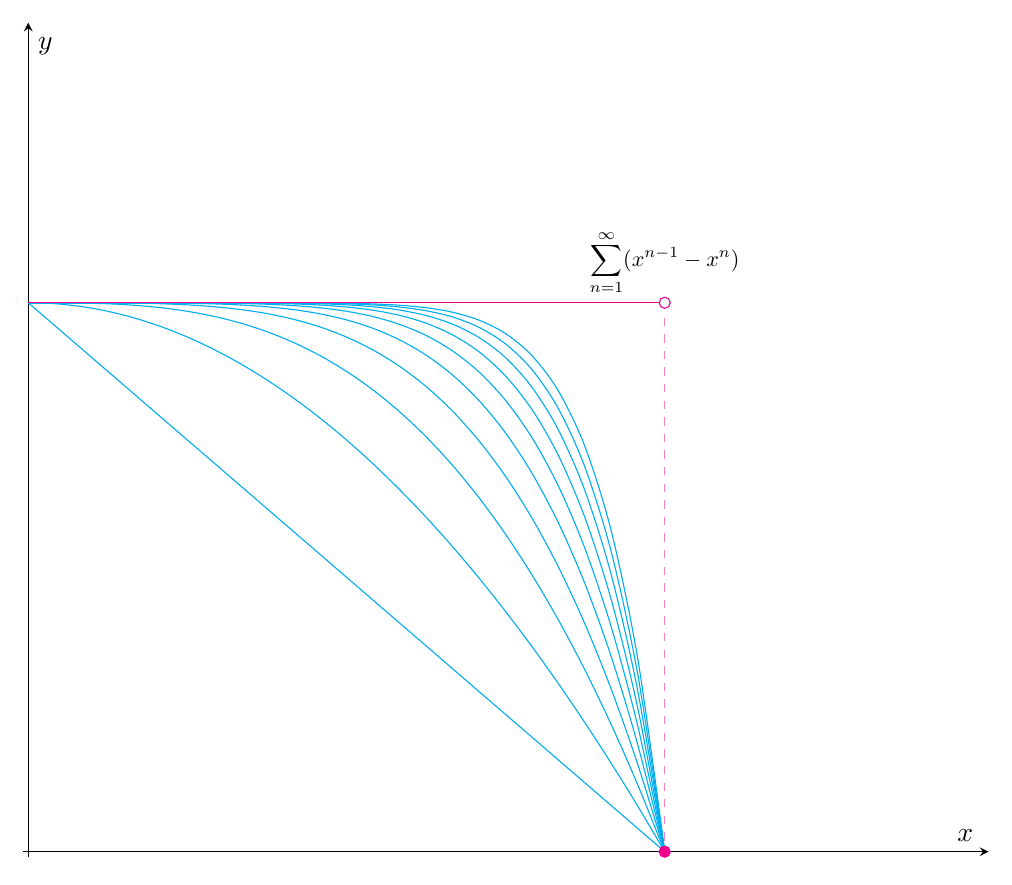
\begin{tikzpicture}[shorten >=-2pt,shorten <=-2pt]
        \begin{axis}[
                ticks=none,
                axis x line=middle,
                axis y line=middle,
                xmin=0, xmax=1.5,
                ymin=0, ymax=1.5,
                domain=0:1,
                xlabel=$x$,
                ylabel=$y$,
                scale only axis,
                width=\textwidth
            ]

            \pgfmathdeclarefunction{un}{1}{\pgfmathparse{1-x^#1}}
            \pgfplotsinvokeforeach{1,...,10}{
                \addplot[color=cyan,smooth] {un(#1)};
            }
            \addplot[color=magenta] {1} node [black,above,scale=0.8] {$\displaystyle\sum_{n=1}^\infty (x^{n-1}-x^{n})$};
            \addplot[color=magenta,only marks,style={mark=*}] coordinates {(1,0)} ;
            \addplot[color=magenta,only marks,style={mark=*, fill=white}] coordinates {(1,1)} ;
            \draw[color=magenta!50!white,dashed] (axis cs:1,0) -- (axis cs:1,1);
        \end{axis}
    \end{tikzpicture}
    \caption{蓝色系列曲线为有限的连续函数相加,而无限个连续函数的和函数为红色曲线,可以看出在$x=1$处不连续。}
\end{marginfigure}
有限个连续函数的和仍是连续函数,但无限个连续函数的和函数即使存在,也未必是连续函数。例如
\[
    (1-x) + (x-x^2) + \cdots + (x^{n-1}-x^n) + \cdots =
    \begin{cases}
        1, & 0\leq x < 1, \\
        0, & x=1
    \end{cases}
\]
对于连续性来说,实际上就是极限与极限符号是否可交换,即下述等式能否成立。
\[
    \lim_{x\to x_0}S(x)
    =
    \lim_{x\to x_0} \lim_{n\to\infty} S_n(x)
    \stackrel{\textcolor{red}{?}}{=}
    \lim_{n\to\infty} \lim_{x\to x_0} S_n(x)
    =
    \lim_{n\to\infty} S_n(x_0)
    =
    S(x_0)
\]
对于求导与积分,也是同理(相应的操作能否与求和符号交换)。

\paragraph{一致收敛}
为了解决和函数的连续性、可导性和可积性问题,因此引入函数项级数的一致收敛概念。
\begin{definition}
    设$S(x),S_n(x)$分别是级数$\displaystyle\sum_{n=1}^\infty u_n(x)$在区间$I$上的和函数与部分和函数,
    如果$\varepsilon > 0,\exists N$,使得当$n>N,x\in I$时,恒有
    \[ \left| S_n(x) - S(x) \right| < \varepsilon \]
    则称$S_n(x)$或级数$\displaystyle\sum_{n=1}^\infty u_n(x)$在区间$I$上一致收敛于$S(x)$
\end{definition}
其实为部分和函数到和函数的距离为无穷小量时,级数一致收敛。

在难以求出和函数的情况下,可以用数列极限的柯西准则\ref{th:柯西准则}判别级数的一致收敛性。即
\[
    \displaystyle\sum_{n=1}^\infty u_n(x)\,(x\in I)\text{ 一致收敛}
    \iff
    \forall \varepsilon >0,\exists N, m>n>N, x\in I, \text{ 恒有} |S_m(x)-S_n(x)|<\varepsilon
\]

要判断函数项级数的一致收敛性,常用方法时构造一个收敛的数项控制级数,只要控制级数收敛,便有被控制级数的一致收敛。
这一方法称为控制判别法。
\begin{theorem}
    (控制判别法)
    \label{th:控制判别法}
    设非负数项级数$\displaystyle\sum_{n=1}^\infty M_n$收敛,如果对所有的$n$和$x\in I$,都有
    $|u_n(x)|\leq M_n$,则$\displaystyle\sum_{n=1}^\infty u_n(x)$在$I$上一致收敛。
\end{theorem}
\begin{proof}
    由于$\displaystyle\sum_{n=1}^\infty M_n$收敛,根据柯西准则,$\forall \varepsilon>0,\exists N$使得当
    $m>n>N$时,恒有部分和片段$\displaystyle\sum_{k>n}^m M_k < \varepsilon$,于是$x\in I$,恒有
    \[ \left| \sum_{k>n}^m u_k(x) \right| \leq \sum_{k>n}^m |u_k(x)| \leq \sum_{k>n}^m M_k < \varepsilon \]
    因此$\displaystyle\sum_{n=1}^\infty u_n(x)$在$I$上一致收敛。
\end{proof}

\begin{example}
    证明$\displaystyle\sum_{n=1}^\infty \frac{\sin nx}{n^2}$在$(-\infty,+\infty)$上一致收敛。
\end{example}
\begin{proof}
    由于在$x\in(-\infty,+\infty)$时,恒有$\dfrac{\sin nx}{n^2} \leq \dfrac{1}{n^2}$,
    而$\displaystyle\sum_{n=1}^\infty \frac{1}{n^2}$收敛,所以原函数项级数在$(-\infty,+\infty)$上一致收敛。
\end{proof}

\begin{example}
    讨论级数$\displaystyle\sum_{n=1}^\infty \frac{1}{n^2}\mathrm{e}^{-nx}$的一致收敛性。
\end{example}
\begin{solution}
    当$x<0$时,$\displaystyle\lim_{n\to\infty} \frac{1}{n^2}\mathrm{e}^{-nx} = +\infty$,原级数发散;

    当$x\geq 0$时,$\dfrac{1}{n^2}\mathrm{e}^{-nx}\leq \dfrac{1}{n^2}$,所以原级数一致收敛。
\end{solution}

\subsection{和函数的性质}
有了一致连续,则可以讨论函数项级数的连续性守恒问题、逐项求导问题、逐项积分问题。
\begin{theorem}
    (和函数的连续性)
    \label{th:和函数的连续性}
    设$\displaystyle\sum_{n=1}^\infty u_n(x)$在区间$I$上一致收敛于$S(x)$,如果每个$u_n(x)$都在$I$上连续,
    则和函数$S(x)$也在$I$上连续。
\end{theorem}
\begin{theorem}
    (和函数的可积性)
    \label{th:和函数的可积性}
    设$\displaystyle\sum_{n=1}^\infty u_n(x)$在区间$[a,b]$上一致收敛于$S(x)$,如果每个$u_n(x)$都在$[a,b]$上连续,
    则和函数$S(x)$在$[a,b]$上可积,且
    \[ \int_a^b S(x)\,\diff x = \sum_{n=1}^\infty \int_a^b u_n(x)\,\diff x \]
\end{theorem}
\begin{theorem}
    (和函数的可微性)
    \label{th:和函数的可微性}
    设$\displaystyle\sum_{n=1}^\infty u_n(x)$在区间$I$上\textcolor{red}{点点收敛}于$S(x)$,如果每个$u_n'(x)$都在$I$上连续,
    则$\displaystyle\sum_{n=1}^\infty u_n'(x)$在区间$I$上一致收敛,则和函数$S(x)$在$I$上可导,且
    \[ S'(x) = \sum_{n=1}^\infty u_n'(x) \]
\end{theorem}
\begin{proof}
    设$a\in I$且$\displaystyle\sum_{n=1}^\infty u_n'(x)$在$I$上一致收敛于$T(x)$,则由\ref{th:和函数的可积性}可知,
    \[
        \int_a^x T(t)\,\diff t
        =
        \sum_{n=1}^\infty \int_a^x u_n'(t)\,\diff t
        =
        \sum_{n=1}^\infty [u_n(x)-u_n(a)]
        =
        S(x) - S(a)
    \]
    所以,$T(x)=S'(x)$,即$\displaystyle S'(x)=\sum_{n=1}^\infty u_n'(x)$
\end{proof}

\section{幂级数}
形如
\[ a_0 + a_1x + a_2x^2 + \cdots + a_nx^n +\cdots \]
的函数项级数称为\textcolor{red}{\textbf{\textsf{幂级数}}}。

\subsection{幂级数的敛散性}
幂级数的收敛域可能是一个区间,也可能退化为一个点。

\begin{theorem}
    (Abel定理)
    \label{th:Abel定理}
    \begin{enumerate}[(1)]
        \item 若幂级数$\displaystyle\sum_{n=0}^\infty a_nx^n$在非零点$a$收敛,则在开区间$(-|a|,|a|)$内绝对收敛。
        \item 若幂级数$\displaystyle\sum_{n=0}^\infty a_nx^n$在非零点$a$发散,则当$|x| > |a|$时,幂级数$\displaystyle\sum_{n=0}^\infty a_nx^n$发散。
    \end{enumerate}
\end{theorem}
\begin{proof}
    由于级数$\displaystyle\sum_{n=0}^\infty a_na^n$收敛,则当$|x| < |a|$时有
    \[ |a_nx^n| = \left|\frac{a_na^n \cdot x^n}{a^n}\right| \leq M\left|\frac{x}{a}\right|^n  \]
    根据根值判别法可知$\displaystyle\sum_{n=0}^\infty M\left|\frac{x}{a}\right|^n$在$|x| < |a|$时收敛,
    所以由比较判别法可知$\displaystyle\sum_{n=0}^\infty |a_nx^n|$收敛。
    即幂级数$\displaystyle\sum_{n=0}^\infty a_nx^n$在开区间$(-|a|,|a|)$内绝对收敛。
\end{proof}
根据Abel定理,幂级数$\displaystyle\sum_{n=0}^\infty a_nx^n$的收敛域有三种情况:
\begin{enumerate}
    \item 单点集$\{0\}$
    \item 全数集$(-\infty,+\infty)$
    \item 有限区间$(-R,R), (-R,R], [-R,R), [-R,-R]$之一
\end{enumerate}
其中$R$为级数的收敛半径。特别称$(-R,R)$为\textcolor{red}{\textbf{\textsf{收敛开区间}}},
简称\textcolor{red}{\textbf{\textsf{收敛区间}}}\sidenote{
    当题目求收敛域时,要考虑端点是否收敛。而求收敛区间时,则无需考虑端点是否收敛。
}。

\begin{theorem}
    (收敛半径)
    如果$\displaystyle\lim_{n\to\infty}\left| \frac{a_{n+1}}{a_n} \right| = l$或$\displaystyle\lim_{n\to\infty}\sqrt[n]{|a_n|}=l$,则幂级数
    $\displaystyle\sum_{n=0}^\infty a_nx^n$的收敛半径为
    \[ R = \lim_{t \to l} \frac{1}{t} \]
\end{theorem}

求收敛域得步骤如下:
\begin{enumerate}[(1)]
    \item 根据比值判别法或根值判别法,求出收敛半径$R$
    \item 若$R=0$或$R=+\infty$,则得出收敛域$\{0\}$、$(-\infty,+\infty)$,否则继续下述步骤
    \item 将$x=R,x=-R$分别带入幂级数,得到数项级数
    \item 若数项级数收敛,则保留端点$R$
    \item 最后得出收敛域。
\end{enumerate}

\begin{example}
    求幂级数$\displaystyle \sum_{n=0}^\infty \frac{1}{3^n}(x-2)^{2n}$的收敛域和收敛半径。
\end{example}
\begin{solution}
    设$t=(x-2)^2$,根据根值判别法
    \[ \lim_{n\to\infty} \sqrt[n]{\frac{1}{3^n}}=\frac{1}{3} \]
    所以收敛半径$R=3$,将$x =\pm 3$带入原幂级数得
    \[ \sum_{n=0}^\infty \frac{1}{3^n} \]
    根据根值判别法可知,级数收敛。
    故有$(x-2)^2 \in [-3,3]$,所以收敛域为$[2-\sqrt{3},2+\sqrt{3}]$
\end{solution}

\begin{theorem}
    (内闭一致收敛性)
    \label{th:内闭一致收敛性}
    若幂级数$\displaystyle\sum_{n=0}^\infty a_nx^n$的收敛半径为$R$且$R>0$,
    则该幂级数在$(-R,R)$的每个闭子区间$[a,b]$上一致收敛。
\end{theorem}
\begin{proof}
    设$r=\max(|a|,|b|)$,则对于$x\in[a,b]$,都有
    \[ |a_nx^n| \leq |a_nr^n| \]
    而由于$0<r<R$,根据Abel定理\ref{th:Abel定理}可知,$\displaystyle\sum_{n=0}^\infty a_nr^n$绝对收敛级数一定收敛。
    根据控制判别法\ref{th:控制判别法}可知,原级数在$(-R,R)$上内闭一致收敛。
\end{proof}

根据幂级数的内闭一致收敛性,幂级数在\textcolor{red}{收敛区间}内的和函数连续,并且可任意此逐项求导和逐项积分,\textcolor{red}{收敛半径始终保持不变}。

数项级数的求和问题通常可以先转化为函数项级数求和问题,再通过分析运算解决(求导后积分、积分后求导)。
\begin{example}
    求级数$1 - \dfrac{1}{3} + \dfrac{1}{5} - \cdots + (-1)^{n+1}\dfrac{1}{2n-1} + \cdots$的和。
\end{example}
\begin{solution}
    设
    \[
        S(x) = x - \frac{1}{3}x^3 + \frac{1}{5}x^5 - \cdots + (-1)^{n+1}\frac{1}{2n-1}x^{2n-1} + \cdots
        =\sum_{n=0}^\infty (-1)^{n+1}\frac{1}{2n-1}x^{2n-1}
    \]
    所以
    \[  \lim_{n\to\infty} \sqrt[n]{|(-1)^{n+1}|} = 1 \]
    所以$S(x)$的收敛半径为$R=1$。

    当$x=1$时
    \[ S(1) = \sum_{n=0}^\infty (-1)^{n+1}\frac{1}{2n-1} \]
    由Leibniz判别法\ref{th:Leibniz判别法},可知$S(1)$收敛;

    当$x=-1$时
    \[ S(-1) = \sum_{n=0}^\infty (-1)^{n}\frac{1}{2n-1} \]
    由Leibniz判别法\ref{th:Leibniz判别法},可知$S(-1)$收敛。

    所以收敛域为$[-1,1]$,在收敛区间$(-1,1)$内,有
    \begin{align*}
        S'(x)
         & = (x)' - \left(\frac{1}{3}x^3\right)' + \left(\frac{1}{5}x^5\right)' - \cdots + \left[(-1)^{n+1}\frac{1}{2n-1}x^{2n-1}\right]' + \cdots \\
         & = 1 - x^2 + x^4 - \cdots + (-1)^{n+1}x^{2n} + \cdots                                                                                    \\
         & = \lim_{n\to\infty} \frac{1\cdot[1-(-1)^nx^{2n}]}{1-(-1)x^2}                                                                            \\
         & = \frac{1}{1+x^2}
    \end{align*}
    于是,
    \[ S(x) = S(x) - S(0)=\int_0^x S'(t)\,\diff t = \int_0^x \frac{1}{1+t^2}\,\diff t = \arctan x \]
    由此可知
    \[ S(1) = \frac{\pi}{4} \]
\end{solution}

\begin{example}
    求幂级数$\displaystyle\sum_{n=0}^infty \frac{(-1)^n}{3n+1}x^{3n}$的收敛域与和函数,
    并求$\displaystyle\sum_{n=0}^\infty\frac{(-1)^n}{3n+1}$
\end{example}
\begin{solution}
    设$t=x^3$,则
    \[
        \lim_{n\to\infty} \left|\frac{a_{n+1}}{a_n}\right|
        =
        \lim_{n\to\infty} \frac{3n+4}{3n+1}
        =
        1
    \]
    所以$|t|<1$,即$x\in(-1,1)$时,幂函数绝对收敛。当$x=1$时,幂级数条件收敛;$x=-1$时,幂级数发散。

    所以幂级数的收敛域为$(-1,1]$,设和函数
    \[ S(x) = \sum_{n=0}^\infty \frac{(-1)^n}{3n+1}x^{3n} \]
    则有$S(0)=1$,当$x\neq 0$时,设$\varphi(x) = xS(x)$,则有
    \begin{align*}
        \varphi(x)  & = \sum_{n=0}^\infty \frac{(-1)^n}{3n+1}x^{3n+1}     \\
        \varphi'(x) & = \sum_{n=0}^\infty (-1)^n x^{3n} = \frac{1}{1+x^3}
    \end{align*}
    所以
    \begin{align*}
        \varphi(x)
         & = \varphi(0) + \int_0^x \varphi'(t)\,\diff t = \int_0^x \frac{1}{1+t^3}\,\diff t                                                                                             \\
         & = \frac{1}{3}\int_0^x \frac{1}{1+t}\,\diff t - \frac{1}{3}\int_0^x \frac{t-2}{t^2-t+1}\,\diff t                                                                              \\
         & = \frac{1}{3}\ln(1+x) - \frac{1}{3}\left( \frac{1}{2}\int_0^x \frac{\diff (t^2-t+1)}{t^2-t+1} - \frac{3}{2}\int_0^x \frac{\diff t}{(t-\frac{1}{2})^2 + \frac{3}{4}}  \right) \\
         & = \frac{1}{3}\ln(1+x) - \frac{1}{6}\ln(x^2-x+1) + \frac{1}{\sqrt{3}}\arctan\frac{2x-1}{\sqrt{3}} +\frac{\pi}{6\sqrt{3}}
    \end{align*}
    于是原幂级数的和函数为
    \[
        S(x) =
        \begin{cases}
            \dfrac{1}{3x}\left[\ln\dfrac{1+x}{\sqrt{x^2-x+1}}+ \sqrt{3}\arctan\dfrac{2x-1}{\sqrt{3}} + \dfrac{\pi}{2\sqrt{3}}\right], & x\in(-1,0)\cup(0,1] \\
            0,                                                                                                                        & x=0
        \end{cases}
    \]
    令$x=1$得,$\displaystyle\sum_{n=0}^\infty\frac{(-1)^n}{3n+1} = \frac{1}{3}\ln 2 + \frac{\pi}{3\sqrt{3}}$
\end{solution}

\begin{example}
    设数列${a_n}$满足$a_1=a_2=1$,且$a_{n+1}=a_n+a_{n-1}, n=2,3,\cdots$,证明在$|x|<\dfrac{1}{2}$时,
    幂级数$\displaystyle\sum_{n=1}^\infty a_nx^{n-1}$收敛,并求其和函数与系数$a_n$。
\end{example}
由于幂级数的收敛类似于$\displaystyle\sum_{n=0}^\infty a^nx^n$
其中$a$与幂级数的收敛半径$R$相关。所以当知道幂级数的收敛区间时,可以令$\dfrac{1}{a}\geq R$,且幂级数$\displaystyle\sum_{n=0}^\infty a^nx^n$收敛。
最后利用比较判别法得出原幂级数的相关性质。
\begin{proof}
    注意到$|x|<\dfrac{1}{2}$,且幂级数$\displaystyle\sum_{n=1}^\infty 2^nx^n$在$|x|<\dfrac{1}{2}$时绝对收敛。
    那么若$|a_n x^n| \leq |2^n x^n|$即$a_n\leq 2^n$成立时,则原幂级数收敛。

    下证$a_n\leq 2^n$,设$b_n=2^n$,则有
    \begin{align*}
        b_{n+1} & = \sum_{i=1}^{n}b_i +1 = b_n + b_{n-1} + \cdots + b_1 + 1 \\
        a_{n+1} & = a_{n} + a_{n-1}
    \end{align*}
    且$a_1 < b_1$。比较易知,$a_{n}<b_{n}$恒成立。
    所以根据比较判别法,原幂级数在$|x|<\dfrac{1}{2}$时,绝对收敛。
    \begin{align*}
        S(x) = \sum_{n=1}^\infty a_nx^{n-1}
         & = a_1 + a_2x + \sum_{n=3}^\infty a_nx^{n-1}                                          \\
         & = a_1 +a_2x +\sum_{n=3}^\infty (a_{n-1}+a_{n-2})x^{n-1}                              \\
         & = a_1 +a_2x +\sum_{n=3}^\infty a_{n-1}x^{n-1} + \sum_{n=3}^\infty a_{n-2}x^{n-1}     \\
         & = a_1 +a_2x +x\sum_{n=2}^\infty a_nx^{n-2} + x^2\sum_{n=1}^\infty a_nx^{n-1}         \\
         & = a_1 +a_2x +x(\sum_{n=1}^\infty a_nx^{n-1} - a_1) + x^2\sum_{n=1}^\infty a_nx^{n-1} \\
         & = a_1 - a_1x +a_2x + (x + x^2)S(x)                                                   \\
    \end{align*}
    所以
    \[ S(x) = \frac{1}{1-x-x^2} \]
    此时将$S(x)$展开为幂级数即可得到$a_n$。
    \begin{align*}
        S(x)
         &
        = -\frac{1}{x^2+x-1}
        = -\frac{1}{\left(x+\frac{1}{2}\right)^2-\frac{5}{4}}
        = -\frac{1}{\left(x+\frac{1+\sqrt{5}}{2}\right)\left(x+\frac{1-\sqrt{5}}{2}\right)}                                                                   \\
         & = \frac{1}{\alpha-\beta}\left(\frac{1}{x+\alpha} - \frac{1}{x+\beta}\right)                                                                        \\
         & = \frac{1}{\alpha-\beta}\left[\frac{1}{\alpha}\left(1 + \frac{x}{\alpha}\right)^{-1} - \frac{1}{\beta}\left(1 + \frac{x}{\beta}\right)^{-1}\right] \\
         & = \frac{1}{\alpha-\beta} \sum_{n=0}^\infty\left[\frac{(-1)^n}{\alpha^{n+1}} - \frac{(-1)^n}{\beta^{n+1}}\right]x^n
    \end{align*}
    其中$\alpha = \dfrac{1+\sqrt{5}}{2},\beta = \dfrac{1-\sqrt{5}}{2}$,所以
    \begin{align*}
        \frac{1}{\alpha-\beta}      & = \frac{1}{\sqrt{5}}                            \\
        \frac{(-1)^n}{\alpha^{n+1}} & = (-1)^n\left(\frac{2}{1+\sqrt{5}}\right)^{n+1} \\
        \frac{(-1)^n}{\beta^{n+1}}  & = -\left(\frac{2}{\sqrt{5}-1}\right)^{n+1}      \\
    \end{align*}
    所以
    \begin{align*}
        S(x)
         & = \frac{1}{\sqrt{5}}\sum_{n=0}^\infty\left[(-1)^n\left(\frac{2}{1+\sqrt{5}}\right)^{n+1} + \left(\frac{2}{\sqrt{5}-1}\right)^{n+1} \right]x^n \\
         & = \frac{1}{\sqrt{5}}\sum_{n=1}^\infty\left[(-1)^{n-1}\left(\frac{2}{1+\sqrt{5}}\right)^n + \left(\frac{2}{\sqrt{5}-1}\right)^n \right]x^{n-1}
    \end{align*}
    由幂级数唯一可知
    \[ a_n = \frac{1}{\sqrt{5}} \left[(-1)^{n-1}\left(\frac{2}{1+\sqrt{5}}\right)^n + \left(\frac{2}{\sqrt{5}-1}\right)^n \right] \]
\end{proof}

\subsection{泰勒级数}
.
\begin{theorem}
    (泰勒级数)
    \label{th:泰勒级数}
    设函数$f(x)$在$|x-x_0|<R$内有各阶导数(无穷阶导数),则$f(x)$在该领域内可展为泰勒级数当且仅当$|x-x_0|<R$时,恒有$\displaystyle\lim_{n\to\infty}R_n(x)=0$
    其中$R_n(x)$为泰勒展开的余项,即
    \[ R_n(x) = f(x) - \sum_{k=0}^{\infty}\frac{f^{(k)}(x_0)}{k!}(x-x_0)^k \]
    此时,有
    \[ f(x) = \sum_{n=0}^\infty \frac{f^{(n)}(x_0)}{n!}(x-x_0)^n \]
    当$x_0=0$时,$f(x)$的泰勒级数称为\textcolor{red}{\textbf{\textsf{麦克劳林级数}}}。
\end{theorem}

余项即为无穷展开减去前面有限的展开,所剩的多项式。
在估计函数值时,所要求的截断误差即为$R_n$,由于$\lim_{n\to\infty}R_n=0$,所以适当增加$n$使得截断误差复合题目即可。
此时前$n$项展开的多项式求和即为估计值。

\begin{example}
    设$f(x)=\dfrac{1}{1-2x-x^2}$
    \begin{enumerate}[(1)]
        \item 将$f(x)$展开为$x$得幂级数;
        \item 分别判断级数$\displaystyle\sum_{n=0}^\infty \frac{n!}{f^{(n)}(0)},\sum_{n=0}^\infty \frac{f^{(n)}(0)}{n!}$得敛散性。
    \end{enumerate}
\end{example}
\begin{solution}
    \begin{enumerate}[(1)]
        \item \begin{align*}
                  f(x) & = -\frac{1}{(x+1)^2-2} = -\frac{1}{(x+1+\sqrt{2})(x+1-\sqrt{2})}                                                                                         \\
                       & = \frac{1}{2\sqrt{2}}\left(\frac{1}{x+1+\sqrt{2}} - \frac{1}{x+1-\sqrt{2}}\right)                                                                        \\
                       & = \frac{1}{2\sqrt{2}}\left(\frac{1}{1+\sqrt{2}}\cdot\frac{1}{1 + \frac{x}{1+\sqrt{2}}}- \frac{1}{1-\sqrt{2}}\cdot\frac{1}{1+\frac{x}{1-\sqrt{2}}}\right) \\
                       & = \frac{1}{2\sqrt{2}}\left[\sum_{n=0}^\infty \frac{(-1)^nx^n}{(1+\sqrt{2})^{n+1}} - \sum_{n=0}^\infty \frac{(-1)^nx^n}{(1-\sqrt{2})^{n+1}}\right]        \\
                       & = \frac{1}{2\sqrt{2}}\sum_{n=0}^\infty\left[\frac{(-1)^n}{(\sqrt{2}+1)^{n+1}} + \frac{1}{(\sqrt{2}-1)^{n+1}}\right]x^n                                   \\
                       & = \frac{1}{2\sqrt{2}}\sum_{n=0}^\infty\left[(-1)^n(\sqrt{2}-1)^{n+1} + (\sqrt{2}+1)^{n+1}\right]x^n
              \end{align*}
        \item 根据麦克劳林展开
              \[ f(x) = \sum_{n=0}^\infty \frac{f^{(n)}(0)}{n!}x^n \]
              的唯一性,比较(1)中的幂级数可得
              \begin{align*}
                  \frac{f^{(n)}(0)}{n!}
                   & = \frac{1}{2\sqrt{2}}\left[(-1)^n(\sqrt{2}-1)^{n+1} + (\sqrt{2}+1)^{n+1}\right]                              \\
                   & = \frac{(\sqrt{2}-1)^{n+1}}{2\sqrt{2}}\left[(-1)^n + \left(\frac{\sqrt{2}+1}{\sqrt{2}-1}\right)^{n+1}\right]
              \end{align*}
              显然$\dfrac{f^{(n)}(0)}{n!}>0$,故$\dfrac{n!}{f^{(n)}(0)}>0$,令$u_n=\dfrac{n!}{f^{(n)}(0)},v_n = \dfrac{1}{(\sqrt{2}+1)^{n+1}}$
              \begin{align*}
                  \lim_{n\to\infty} \frac{u_n}{v_n}
                   & = \lim_{n\to\infty} \frac{2\sqrt{2}(\sqrt{2}+1)^{n+1}}{(-1)^n(\sqrt{2}-1)^{n+1} + (\sqrt{2}+1)^{n+1}}     \\
                   & = 2\sqrt{2}\lim_{n\to\infty} \left[(-1)^n\left(\frac{\sqrt{2}-1}{\sqrt{2}+1}\right)^{n+1} + 1\right]^{-1} \\
                   & = 2\sqrt{2}
              \end{align*}
              又级数$\displaystyle\sum_{n=0}^\infty v_n$收敛,所以由极限判别法可知,级数$\displaystyle\sum_{n=0}^\infty \frac{n!}{f^{(n)}(0)}$收敛,
              则有\[\lim_{n\to\infty} \frac{n!}{f^{(n)}(0)} = 0,\qquad \lim_{n\to\infty} \frac{f^{(n)}(0)}{n!} =\infty \]
              所以级数$\displaystyle\sum_{n=0}^\infty \frac{f^{(n)}(0)}{n!}$发散。

    \end{enumerate}
\end{solution}

\section{傅里叶级数}
\subsection{\texorpdfstring{$2\pi$}{2π}周期的傅里叶级数}
形如
\begin{equation}
    \frac{a_0}{2} + \sum_{n=1}^\infty(a_n\cos nx + b_n\sin nx)
\end{equation}
的函数项级数称为\textcolor{red}{\textbf{\textsf{三角级数}}},其中$a_0,a_1,b_1,\cdots$称为三角级数的系数。

\subsubsection{三角函数系的正交性}
构成三角级数的函数系
\[ 1,\cos x,\sin x,\cdots,\cos nx, \sin nx \]
在区间$[a,b]$上定义内积运算
\begin{equation}
    \langle f(x),g(x) \rangle  = \int_a^b f(x)g(x)\,\diff x
\end{equation}
即将$f(x)$看作在区间$[a,b]$上的无穷维向量$(f(x_1),f(x_2),\cdots)$,$g(x)$同理,
则向量的内积为$f(x_1)g(x_1)+f(x_2)g(x_2)+\cdots = \int_a^b f(x)g(x)\,\diff x$


在区间$[-\pi,\pi]$上,三角函数系具有正交性,即函数系中仍以两个不同函数按照,的内积都为零。
而相同函数的内积为
\[
    \langle 1,1 \rangle = 2\pi;\,
    \langle \cos nx, \cos nx \rangle
    =
    \langle \sin nx, \sin nx\rangle
    =
    \pi
\]

\subsubsection{函数的傅里叶展开}
如果函数$f(x)$在$[-\pi,\pi]$上可以展开为三角级数,或则说三角级数在$[-\pi,\pi]$收敛于$f(x)$,即
\begin{equation}
    f(x) = \frac{a_0}{2} + \sum_{n=1}^\infty (a_n\cos nx + b_n \sin nx)
\end{equation}
则在\textcolor{red}{逐项可积}的条件下,由三角函数系得正交性可以推出
\begin{align}
    a_0 & = \frac{1}{\pi}\langle f(x),1 \rangle        = \frac{1}{\pi}\int_{-\pi}^{\pi} f(x)\,\diff x        \\
    a_n & = \frac{1}{\pi}\langle f(x),\cos nx \rangle  = \frac{1}{\pi}\int_{-\pi}^{\pi} f(x)\cos nx\,\diff x \\
    b_n & = \frac{1}{\pi}\langle f(x),\sin nx \rangle  = \frac{1}{\pi}\int_{-\pi}^{\pi} f(x)\sin nx\,\diff x
\end{align}

若$f(x)$是以$2\pi$为周期,由于三角函数系周期也是$2\pi$,则当$f(x)$给出在区间$[0,2\pi]$上的表达式时,
可以直接将傅里叶系数的计算积分上下限直接改为$[0,2\pi]$,其原因是$f(x)$与三角函数系的乘积仍以$2\pi$为周期,
同时周期为$T$的函数定积分有
\[ \int_a^{a+T} f(x)\,\diff x = \int_0^T f(x)\,\diff x \]

\begin{theorem}
    (Dirichlet收敛定理)
    \label{th:Dirichlet收敛定理}
    若函数$f(x)$在$[-\pi,\pi]$上满足Dirichlet条件:
    \begin{enumerate}[(1)]
        \item 最多只有有限个第一类间断点
        \item 最多只有有限阿极值点
    \end{enumerate}
    则函数$f(x)$的傅里叶级数收敛。且有
    \begin{enumerate}[(1)]
        \item 当$x$是$f(x)$的连续点时,级数收敛于$f(x)$;
        \item 当$x$是$f(x)$的间断点时,级数收敛于$\dfrac{f(x^-)+f(x^+)}{2}$;
        \item 当$x=\pm\pi$时,级数收敛于$\dfrac{f(-\pi^+)+f(\pi^-)}{2}$
    \end{enumerate}
\end{theorem}

函数展开称为傅里叶级数的条件比展开成幂级数的条件\textcolor{red}{弱}得多,只要函数在区间$[-\pi,\pi]$上不作无限次振荡,
间断点个数有限且左右极限存在,则函数在连续点收敛到函数值,在间断点收敛到左右极限得平均值。

\begin{example}
    设函数$f(x)$时以$2\pi$为周期的周期函数,且$f(x)=\mathrm{e}^{\alpha x}\,(0\leq x<2\pi)$,
    其中$\alpha\neq 0$,试将$f(x)$展开成傅里叶级数,并求级数$\displaystyle\sum_{n=1}^\infty\frac{1}{1+n^2}$的和。
\end{example}
\begin{solution}
    \[ a_0 = \frac{1}{\pi}\int_0^{2\pi} f(x)\,\diff x = \frac{\mathrm{e}^{2\alpha\pi} - 1}{\alpha\pi}\]
    \begin{align*}
        a_n & = \frac{1}{\pi}\int_0^{2\pi} f(x)\cos nx\,\diff x = \frac{1}{\pi}\int_0^{2\pi} \mathrm{e}^{\alpha x}\cos nx\,\diff x                         \\
            & =\frac{1}{\alpha\pi} \left(\left.\mathrm{e}^{\alpha x}\cos nx\right|_0^{2\pi} + n\int_0^{2\pi} \mathrm{e}^{\alpha x}\sin nx\,\diff x \right) \\
            & =\frac{\mathrm{e}^{2\alpha\pi} - 1}{\alpha\pi} +  \frac{n}{\alpha}b_n
    \end{align*}
    \begin{align*}
        b_n & = \frac{1}{\pi}\int_0^{2\pi} f(x)\sin nx\,\diff x = \frac{1}{\pi}\int_0^{2\pi} \mathrm{e}^{\alpha x}\sin nx\,\diff x                         \\
            & =\frac{1}{\alpha\pi} \left(\left.\mathrm{e}^{\alpha x}\sin nx\right|_0^{2\pi} - n\int_0^{2\pi} \mathrm{e}^{\alpha x}\cos nx\,\diff x \right) \\
            & =-\frac{n}{\alpha}a_n
    \end{align*}
    联立两式得
    \begin{align*}
        a_n & = \frac{\mathrm{e}^{2\alpha\pi}-1}{\pi} \cdot \frac{\alpha}{\alpha^2+n^2} \\
        b_n & = -\frac{\mathrm{e}^{2\alpha\pi}-1}{\pi} \cdot \frac{n}{\alpha^2+n^2}
    \end{align*}
    因此
    \[
        f(x) = \mathrm{e}^{\alpha x}
        = \frac{\mathrm{e}^{2\alpha\pi} - 1}{\pi}
        \left(\frac{1}{2\alpha} + \sum_{n=1}^\infty \frac{\alpha\cos nx - n\sin nx}{\alpha^2+n^2}\right)
    \]
    令$\alpha=1,x=0$,根据Dirichlet定理可知
    \[
        \frac{\mathrm{e}^{2\pi} - 1}{\pi}\left(\frac{1}{2}+ \sum_{n=1}^\infty \frac{1}{1+n^2}\right)
        =
        \frac{f(0^+)+f(2\pi^-)}{2}
        =
        \frac{1+\mathrm{e}^{2\pi}}{2}
    \]
    则级数
    \[ \sum_{n=1}^\infty \frac{1}{1+n^2} = \frac{\pi}{2}\cdot\frac{\mathrm{e}^{2\pi}+1}{\mathrm{e}^{2\pi}-1} - \frac{1}{2} \]
\end{solution}


\subsection{一般周期得傅里叶级数}
有时需要将函数展为正弦级数或余弦级数,又是还需要在区间$[-l,l]$上将函数展为傅里叶级数,这些情况只要作一些简单的数学处理,
如函数的奇延拓、偶延拓或线性变换,即可化为$[-\pi,\pi]$上的傅里叶展开问题。

\begin{theorem}
    如果函数$f(x)$在$[0,\pi]$上可以展为正弦函数
    \[ f(x) = b_1\sin x + b_2\sin 2x + \cdots + b_n \sin nx + \cdots \]
    则有
    \[ b_n = \frac{2}{\pi}\int_0^\pi f(x)\sin nx \,\diff x \]

    如果函数$f(x)$在$[0,\pi]$上可以展为余弦函数
    \[ f(x) = \frac{a_0}{2} + a_1\cos x + a_2\cos 2x + \cdots + a_n \cos nx + \cdots \]
    则有
    \[ a_n = \frac{2}{\pi}\int_0^\pi f(x)\cos nx \,\diff x \]
\end{theorem}
\begin{proof}
    令
    \[
        F(x) =
        \begin{cases}
            f(x),   & 0<x\leq\pi     \\
            0,      & x=0            \\
            -f(-x), & -\pi\leq x < 0
        \end{cases},
        \qquad
        G(x) =
        \begin{cases}
            f(x),  & 0\leq x \leq \pi \\
            f(-x), & \pi \leq x < 0
        \end{cases}
    \]
    即对$f(x)$分别进行奇延拓、偶延拓。在$[-\pi,\pi]$上分别计算$F(x),G(x)$的傅里叶系数可证原命题。
\end{proof}

\begin{theorem}
    如果函数$f(x)$在$[-l,l]$上可以展为傅里叶级数
    \[ f(x) = \frac{a_0}{2} + \sum_{n=1}^\infty(a_n\cos \frac{n\pi x}{l} + b_n\sin\frac{n\pi x}{l}) \]
    则有
    \begin{align*}
        a_n & = \frac{1}{l}\int_{-l}^l f(x)\cos\frac{n\pi x}{l}\,\diff x (n=0,1,2,\cdots); \\
        b_n & = \frac{1}{l}\int_{-l}^l f(x)\sin\frac{n\pi x}{l}\,\diff x (n=1,2,3,\cdots);
    \end{align*}
\end{theorem}
\begin{proof}
    令$F(x)=\frac{lx}{\pi}$,在$[-\pi,\pi]$上,计算$F(x)$的傅里叶系数可证原命题。
\end{proof}